\documentclass[]{article}
\usepackage{lmodern}
\usepackage{amssymb,amsmath}
\usepackage{ifxetex,ifluatex}
\usepackage{fixltx2e} % provides \textsubscript
\ifnum 0\ifxetex 1\fi\ifluatex 1\fi=0 % if pdftex
  \usepackage[T1]{fontenc}
  \usepackage[utf8]{inputenc}
\else % if luatex or xelatex
  \ifxetex
    \usepackage{mathspec}
    \usepackage{xltxtra,xunicode}
  \else
    \usepackage{fontspec}
  \fi
  \defaultfontfeatures{Mapping=tex-text,Scale=MatchLowercase}
  \newcommand{\euro}{€}
\fi
% use upquote if available, for straight quotes in verbatim environments
\IfFileExists{upquote.sty}{\usepackage{upquote}}{}
% use microtype if available
\IfFileExists{microtype.sty}{%
\usepackage{microtype}
\UseMicrotypeSet[protrusion]{basicmath} % disable protrusion for tt fonts
}{}
\usepackage[margin=1in]{geometry}
\usepackage{color}
\usepackage{fancyvrb}
\newcommand{\VerbBar}{|}
\newcommand{\VERB}{\Verb[commandchars=\\\{\}]}
\DefineVerbatimEnvironment{Highlighting}{Verbatim}{commandchars=\\\{\}}
% Add ',fontsize=\small' for more characters per line
\usepackage{framed}
\definecolor{shadecolor}{RGB}{248,248,248}
\newenvironment{Shaded}{\begin{snugshade}}{\end{snugshade}}
\newcommand{\KeywordTok}[1]{\textcolor[rgb]{0.13,0.29,0.53}{\textbf{{#1}}}}
\newcommand{\DataTypeTok}[1]{\textcolor[rgb]{0.13,0.29,0.53}{{#1}}}
\newcommand{\DecValTok}[1]{\textcolor[rgb]{0.00,0.00,0.81}{{#1}}}
\newcommand{\BaseNTok}[1]{\textcolor[rgb]{0.00,0.00,0.81}{{#1}}}
\newcommand{\FloatTok}[1]{\textcolor[rgb]{0.00,0.00,0.81}{{#1}}}
\newcommand{\CharTok}[1]{\textcolor[rgb]{0.31,0.60,0.02}{{#1}}}
\newcommand{\StringTok}[1]{\textcolor[rgb]{0.31,0.60,0.02}{{#1}}}
\newcommand{\CommentTok}[1]{\textcolor[rgb]{0.56,0.35,0.01}{\textit{{#1}}}}
\newcommand{\OtherTok}[1]{\textcolor[rgb]{0.56,0.35,0.01}{{#1}}}
\newcommand{\AlertTok}[1]{\textcolor[rgb]{0.94,0.16,0.16}{{#1}}}
\newcommand{\FunctionTok}[1]{\textcolor[rgb]{0.00,0.00,0.00}{{#1}}}
\newcommand{\RegionMarkerTok}[1]{{#1}}
\newcommand{\ErrorTok}[1]{\textbf{{#1}}}
\newcommand{\NormalTok}[1]{{#1}}
\usepackage{longtable,booktabs}
\usepackage{graphicx}
\makeatletter
\def\maxwidth{\ifdim\Gin@nat@width>\linewidth\linewidth\else\Gin@nat@width\fi}
\def\maxheight{\ifdim\Gin@nat@height>\textheight\textheight\else\Gin@nat@height\fi}
\makeatother
% Scale images if necessary, so that they will not overflow the page
% margins by default, and it is still possible to overwrite the defaults
% using explicit options in \includegraphics[width, height, ...]{}
\setkeys{Gin}{width=\maxwidth,height=\maxheight,keepaspectratio}
\ifxetex
  \usepackage[setpagesize=false, % page size defined by xetex
              unicode=false, % unicode breaks when used with xetex
              xetex]{hyperref}
\else
  \usepackage[unicode=true]{hyperref}
\fi
\hypersetup{breaklinks=true,
            bookmarks=true,
            pdfauthor={},
            pdftitle={HMM para reconocimiento de vocales},
            colorlinks=true,
            citecolor=blue,
            urlcolor=blue,
            linkcolor=magenta,
            pdfborder={0 0 0}}
\urlstyle{same}  % don't use monospace font for urls
\setlength{\parindent}{0pt}
\setlength{\parskip}{6pt plus 2pt minus 1pt}
\setlength{\emergencystretch}{3em}  % prevent overfull lines
\setcounter{secnumdepth}{5}

%%% Use protect on footnotes to avoid problems with footnotes in titles
\let\rmarkdownfootnote\footnote%
\def\footnote{\protect\rmarkdownfootnote}

%%% Change title format to be more compact
\usepackage{titling}
\setlength{\droptitle}{-2em}
  \title{HMM para reconocimiento de vocales}
  \pretitle{\vspace{\droptitle}\centering\huge}
  \posttitle{\par}
  \author{}
  \preauthor{}\postauthor{}
  \predate{\centering\large\emph}
  \postdate{\par}
  \date{18/05/2015}




\begin{document}

\maketitle


{
\hypersetup{linkcolor=black}
\setcounter{tocdepth}{2}
\tableofcontents
}
\pagebreak

\section{Introducción}\label{introduccion}

Los HMM han sido ampliamente utilizados en problemas de Procesamiento de
Lenguaje Natural (NLP) sobre todo para el etiquetado de partes del habla
(POS) Stamp (2012)

\section{Objetivo}\label{objetivo}

Identificación de vocales y consonantes a través de un modelo de HMM
estimando sus parámetros.

\section{Especificación del modelo}\label{especificacion-del-modelo}

\begin{itemize}
\itemsep1pt\parskip0pt\parsep0pt
\item
  Utilizamos HMM con el algoritmo Baum-Welch para estimar los
  parámetros:
\end{itemize}

\begin{enumerate}
\def\labelenumi{\arabic{enumi}.}
\itemsep1pt\parskip0pt\parsep0pt
\item
  las probabilidades inciales de los estados
\item
  las probabilidades de transición entre estados
\item
  las probabilidades de cada símbolo de pertenecer a uno de los estados
\end{enumerate}

\begin{figure}[htbp]
\centering
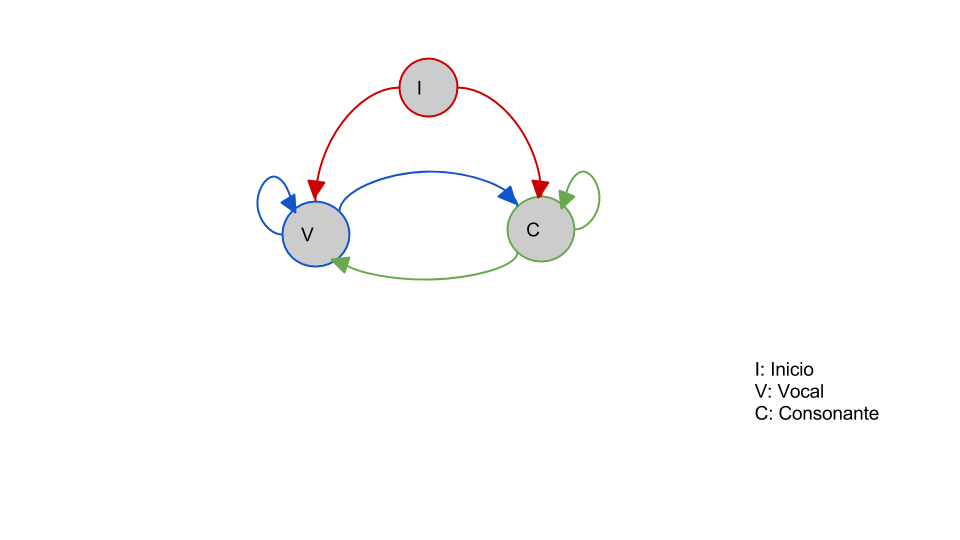
\includegraphics{modelo_vocales.png}
\caption{imagen}
\end{figure}

\subsection{Algoritmo Baum-Welch}\label{algoritmo-baum-welch}

\begin{itemize}
\itemsep1pt\parskip0pt\parsep0pt
\item
  Este algoritmo es una variante del EM visto en clase Frazzoli (2010);
  Bilmes (1998) . Iniciamos con un modelo sin `conocimiento'
\end{itemize}

\(\pi\) = probabilidades de iniciar en cada estado

T= matriz de transición de estados

M= matriz de emisiones

\(\lambda=(T,M,\pi)\)

\begin{itemize}
\itemsep1pt\parskip0pt\parsep0pt
\item
  En cada iteración los valores de \(\pi\), A y B se van actualizando
  hasta convergencia implementando el algoritmo forward-backward.
\end{itemize}

Definimos \(\gamma_{k}(s)=Pr[X_{k}= s|Z,\lambda]\), la probabilidad de
que el sistema se encuentre en el estado \(s\) en el \(k\)-ésimo tiempo,
dada la secuencia de observaciones \(Z\) en el modelo \(\lambda\)
(forward-process).

\(\gamma_{k}(s)=\frac{\alpha_{k}(s)\beta_{k}(s)}{Pr[Z|\lambda]}=\alpha_{k}(s)\beta_{k}(s){\sum_{s\epsilon\chi}\alpha_{t}(s)}\)

Definimos \(\xi_{k}(q,s)=Pr[X_{k}=q,X_{k+1}=s|Z,\lambda]\), la
probabilidad de estar en el estado \(q\) al tiempo \(k\) y en el estado
\(s\) en el tiempo \(k+1\) dada la secuencia de observaciones en el
modelo actual de HMM (backward-process).

\(\xi_{k}(q,s)=\eta_{k}\alpha_{k}(q)T_{q,s}M_{s,z_{k+1}}\beta_{k+1}(s)\),
donde \(\eta_{k}\) es un factor de normalización tal que
\(\sum_{q,s}\xi_{k}(q,s)=1\)

Calculando \(\gamma_{k}(s)\) y \(\xi_{k}(q,s)\) podemos actualizar el
modelo \(\lambda'=(T',M',\pi')\)

\(\pi'_{s}=\gamma_{1}(s)\)

\(T'_{q,s}=\frac{E[\# de transiciones del estado q al s]}{E[\# de transiciones del estado q]}=\frac{\sum_{k=1}^{t-1}\xi_{k(q,s)}}{\sum_{k=1}^{t-1}\gamma_{k}(q)}\)

\(M'_{s,m}=\frac{E[\# de veces en el estado s cuando la observacion fue m]}{E[\# de veces en el estado s]}=\frac{\sum_{k=1}{t}\gamma_{k}(s)1(z_{k}=m)}{\sum_{k=1}^{t}\gamma_{k}(s)}\)

\subsection{~Suposiciones iniciales del
modelo}\label{suposiciones-iniciales-del-modelo}

\begin{itemize}
\itemsep1pt\parskip0pt\parsep0pt
\item
  Nuestra base será suponer que existen 2 estados: \textbf{Consonante} y
  \textbf{Vocal}\\
\item
  No conocemos con qué probabilidad de inicio estamos en Constante o en
  Vocal
\item
  No conocemos las probabilidades de transición entre estados
\item
  No conocemos las probabilidades de que cada símbolo del lenguaje
  pertenezca a uno de los estados
\end{itemize}

\section{~Datos}\label{datos}

Intentamos ocupar los últimos 100 contenidos publicados en Quién.com y
CNNExpansión.com sin embargo sus corpus requieren de mucho de
preprocesamiento para eliminar encoding y caracteres extraños.

Decidimos tomar un corpus en español de un ejercicio realizado en
Métodos Analíticos correspondiente a un periodico español con 309,918
noticias

\subsection{~Limpieza de Datos}\label{limpieza-de-datos}

\begin{itemize}
\itemsep1pt\parskip0pt\parsep0pt
\item
  Eliminamos signos de puntuación
\item
  Eliminamos dígitos
\item
  Eliminamos tabulaciones
\item
  Cambiamos todo el corpus a minúsculas
\item
  Dividimos cada palabra en sus letras respetando los espacios
\end{itemize}

\section{~Metodología}\label{metodologia}

\begin{enumerate}
\def\labelenumi{\arabic{enumi}.}
\itemsep1pt\parskip0pt\parsep0pt
\item
  Limpieza de datos
\item
  Separar cada palabra en sus respectivas letras respetando espacios
\item
  Establecemos nuestro conocimiento a priori sobre las probabilidades
  iniciales de estados inicializando \(\pi\). Dado que no conocemos
  mucho del proceso las establecemos muy cercanas a 0.5 (suman a 1)
\item
  Establecemos nuestro conocimiento a priori sobre las probabilidades de
  transición entre estados inicializando A. Dado que no conocemos mucho
  del proceso las establecemos cercanas a 0.5 pero agregando que creemos
  que es más probable la transición de vocal a consonante que de vocal a
  vocal, al igual que de consonante a vocal de que de consontante a
  consonante.
\item
  Establecemos nuestro conocimiento a priori sobre las probabilidades de
  cada símbolo a cada uno de los estados propuestos inicializando B.
  Dado que no conocemos mucho del proceso las establecemos dividiendo 1
  entre el número de símbolos posibles en el set de datos.
\item
  Inicialización de la HMM con los parámetros establecidos en el paso
  4,5 y 6.
\item
  Correr el algoritmo de Baum-Welch
\end{enumerate}

\section{Paquetes utlizadas}\label{paquetes-utlizadas}

\begin{itemize}
\item
  Paquete HMM de R Himmelmann (2010)
\item
  Algoritmo de Baum-Welch para estimación de parámetros de una HMM
\end{itemize}

\section{Resultados}\label{resultados}

Inicial sin conocimiento:

\begin{longtable}[c]{@{}ccc@{}}
\toprule
& V & C\tabularnewline
\midrule
\endhead
& 0.5337 & 0.4662\tabularnewline
\bottomrule
\end{longtable}

Inicial después de Baum-Welch

\begin{longtable}[c]{@{}ccc@{}}
\toprule
& V & C\tabularnewline
\midrule
\endhead
& 0.5337 & 0.4662\tabularnewline
\bottomrule
\end{longtable}

Transiciones sin conocimiento

\begin{longtable}[c]{@{}ccc@{}}
\toprule
& V & C\tabularnewline
\midrule
\endhead
V & 0.3099 & 0.6900\tabularnewline
C & 0.5200 & 0.4799\tabularnewline
\bottomrule
\end{longtable}

Transiciones después de Baum-Welch

\begin{longtable}[c]{@{}ccc@{}}
\toprule
& V & C\tabularnewline
\midrule
\endhead
V & 0.3045 & 0.6954\tabularnewline
C & 0.993 & 0.006\tabularnewline
\bottomrule
\end{longtable}

\begin{figure}[htbp]
\centering
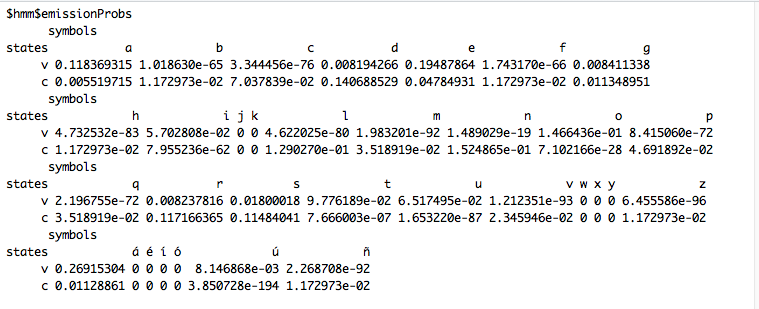
\includegraphics{salida_vocales.png}
\caption{resultados}
\end{figure}

\pagebreak

\section{Código}\label{codigo}

\begin{Shaded}
\begin{Highlighting}[]
\KeywordTok{library}\NormalTok{(HMM)}

\NormalTok{periodico <-}\StringTok{ }\KeywordTok{scan}\NormalTok{(}\DataTypeTok{file=}\StringTok{'./datos/Es_Newspapers.txt'}\NormalTok{, }\DataTypeTok{sep=}\StringTok{"}\CharTok{\textbackslash{}n}\StringTok{"}\NormalTok{, }\DataTypeTok{what =} \KeywordTok{character}\NormalTok{())}

\CommentTok{#limpieza de datos}
\NormalTok{for(i in }\DecValTok{1}\NormalTok{:}\KeywordTok{length}\NormalTok{(periodico)) \{}
  \NormalTok{periodico[i] <-}\StringTok{ }\KeywordTok{gsub}\NormalTok{(}\StringTok{"[[:punct:]]"}\NormalTok{,}\StringTok{""}\NormalTok{,}\KeywordTok{unlist}\NormalTok{(periodico[i]))}
  \NormalTok{periodico[i] <-}\StringTok{ }\KeywordTok{gsub}\NormalTok{(}\StringTok{"[[:digit:]]"}\NormalTok{,}\StringTok{""}\NormalTok{,}\KeywordTok{unlist}\NormalTok{(periodico[i]))}
  \NormalTok{periodico[i] <-}\StringTok{ }\KeywordTok{tolower}\NormalTok{(periodico[i])}
  \NormalTok{periodico[i] <-}\StringTok{ }\KeywordTok{gsub}\NormalTok{(}\StringTok{"[[:space:]]"}\NormalTok{,}\StringTok{" "}\NormalTok{,}\KeywordTok{unlist}\NormalTok{(periodico[i]))}
\NormalTok{\}}


\CommentTok{#separando a letras}
\NormalTok{for (i in }\DecValTok{1}\NormalTok{) \{}
  \NormalTok{texto <-}\StringTok{ }\NormalTok{periodico[i]}
  \NormalTok{if(i ==}\StringTok{ }\DecValTok{1}\NormalTok{)\{}
    \NormalTok{obsv <-}\StringTok{ }\KeywordTok{as.data.frame}\NormalTok{(}\KeywordTok{unlist}\NormalTok{(}\KeywordTok{strsplit}\NormalTok{(texto, }\DataTypeTok{split=}\StringTok{""}\NormalTok{)), }\DataTypeTok{stringsAsFactors=}\OtherTok{FALSE}\NormalTok{)}
  \NormalTok{\} else \{}
    \NormalTok{obsv <-}\StringTok{ }\KeywordTok{rbind}\NormalTok{(obsv, }\KeywordTok{as.data.frame}\NormalTok{(}\KeywordTok{unlist}\NormalTok{(}\KeywordTok{strsplit}\NormalTok{(texto, }\DataTypeTok{split=}\StringTok{""}\NormalTok{)), }\DataTypeTok{stringsAsFactors=}\OtherTok{FALSE}\NormalTok{))}
  \NormalTok{\}}
\NormalTok{\}}
\KeywordTok{names}\NormalTok{(obsv) <-}\StringTok{ "letter"}


\NormalTok{states =}\StringTok{ }\KeywordTok{c}\NormalTok{(}\StringTok{"v"}\NormalTok{,}\StringTok{"c"}\NormalTok{)}
\NormalTok{symbols =}\StringTok{ }\KeywordTok{c}\NormalTok{(}\StringTok{"a"}\NormalTok{,}\StringTok{"b"}\NormalTok{,}\StringTok{"c"}\NormalTok{,}\StringTok{"d"}\NormalTok{,}\StringTok{"e"}\NormalTok{,}\StringTok{"f"}\NormalTok{,}\StringTok{"g"}\NormalTok{,}\StringTok{"h"}\NormalTok{,}\StringTok{"i"}\NormalTok{,}\StringTok{"j"}\NormalTok{,}\StringTok{"k"}\NormalTok{,}\StringTok{"l"}\NormalTok{,}\StringTok{"m"}\NormalTok{,}\StringTok{"n"}\NormalTok{,}\StringTok{"o"}\NormalTok{,}\StringTok{"p"}\NormalTok{,}\StringTok{"q"}\NormalTok{,}\StringTok{"r"}\NormalTok{,}
            \StringTok{"s"}\NormalTok{,}\StringTok{"t"}\NormalTok{,}\StringTok{"u"}\NormalTok{,}\StringTok{"v"}\NormalTok{,}\StringTok{"w"}\NormalTok{,}\StringTok{"x"}\NormalTok{,}\StringTok{"y"}\NormalTok{,}\StringTok{"z"}\NormalTok{,}\StringTok{" "}\NormalTok{,}\StringTok{"á"}\NormalTok{,}\StringTok{"é"}\NormalTok{,}\StringTok{"í"}\NormalTok{,}\StringTok{"ó"}\NormalTok{,}\StringTok{"ú"}\NormalTok{,}\StringTok{"ñ"}\NormalTok{)}
\CommentTok{#probabilidades iniciales de lso estados}
\NormalTok{random_num <-}\StringTok{ }\KeywordTok{runif}\NormalTok{(}\DecValTok{1}\NormalTok{,}\FloatTok{0.5}\NormalTok{,}\FloatTok{0.7}\NormalTok{)}
\NormalTok{startProbs =}\StringTok{ }\KeywordTok{matrix}\NormalTok{(}\KeywordTok{c}\NormalTok{(random_num, }\DecValTok{1}\NormalTok{-random_num), }\DecValTok{2}\NormalTok{)}

\NormalTok{random_num <-}\StringTok{ }\KeywordTok{runif}\NormalTok{(}\DecValTok{1}\NormalTok{, }\FloatTok{0.5}\NormalTok{,}\FloatTok{0.7}\NormalTok{)}
\NormalTok{random_num_2 <-}\StringTok{ }\KeywordTok{runif}\NormalTok{(}\DecValTok{1}\NormalTok{, }\FloatTok{0.5}\NormalTok{,}\FloatTok{0.7}\NormalTok{)}
\NormalTok{transProbs <-}\StringTok{ }\KeywordTok{matrix}\NormalTok{(}\KeywordTok{c}\NormalTok{(}\DecValTok{1}\NormalTok{-random_num, random_num_2, }
                       \NormalTok{random_num, }\DecValTok{1}\NormalTok{-random_num_2), }\DecValTok{2}\NormalTok{)}
  
\NormalTok{random_nums <-}\StringTok{ }\KeywordTok{data.frame}\NormalTok{(}\KeywordTok{runif}\NormalTok{(}\DecValTok{33}\NormalTok{,}\FloatTok{0.030}\NormalTok{,}\FloatTok{0.034}\NormalTok{), }\KeywordTok{runif}\NormalTok{(}\DecValTok{33}\NormalTok{,}\FloatTok{0.030}\NormalTok{,}\FloatTok{0.034}\NormalTok{))}
\NormalTok{random_nums <-}\StringTok{ }\KeywordTok{data.frame}\NormalTok{(}\KeywordTok{rep}\NormalTok{(}\DecValTok{1}\NormalTok{/}\DecValTok{33}\NormalTok{,}\DecValTok{33}\NormalTok{), }\KeywordTok{rep}\NormalTok{(}\DecValTok{1}\NormalTok{/}\DecValTok{33}\NormalTok{,}\DecValTok{33}\NormalTok{))}
\NormalTok{emissionProbs=}\KeywordTok{as.matrix}\NormalTok{(random_nums)}
\NormalTok{inithmm <-}\StringTok{ }\KeywordTok{initHMM}\NormalTok{(states, symbols, }\DataTypeTok{startProbs=}\NormalTok{startProbs, }\DataTypeTok{transProbs=}\NormalTok{transProbs, }
                   \DataTypeTok{emissionProbs=}\NormalTok{emissionProbs)}
\NormalTok{bw <-}\StringTok{ }\KeywordTok{baumWelch}\NormalTok{(inithmm, obsv$letter)}
\NormalTok{bw}
\end{Highlighting}
\end{Shaded}

\pagebreak

\section{Bibliografía}\label{bibliografia}

\end{document}
